\documentclass{article}

\usepackage{amsmath}
\usepackage{amsfonts}
\usepackage{amssymb}
\usepackage{xcolor}
\usepackage{hyperref}
\usepackage{parskip}
\usepackage{a4wide}
\usepackage{graphicx}

\graphicspath{{C:/Users/Jack G/Documents/LaTex/images/}}

\setlength{\parindent}{0pt}
\setlength{\parskip}{1em}

\begin{document}

\section*{AMM LP Greeks}

\subsection*{Summary}

Below I'm going to look at some of the greeks for an AMM LP position and how we can think about hedging them. I'm making a few simplifying assumptions throughout:

\begin{itemize}
\item Trading costs and borrow costs are ignored
\item PnL is in one of the coins staked, assumed to be USDC - analysis of `cross-pair' LPs is coming later as these involve correlation
\item Constant-product AMMs and also UniSwap V3 style concentrated liquidity AMMs are considered
\end{itemize}

Throughout I'll use ETH-USDC as an example pair.

\subsection*{Delta Hedging}
\label{sec:delta}

We have $C(0)$ capital in coin $Y$ (ie. USDC, our PnL measure) that we wish to invest in an LP token. We first exchange half of this into coin $X$ (ie. ETH) at price $p(0)$, and then provide both of these coins in exchange for the LP tokens.

As the ETH price moves around and the size of the pools vary, we will pick up Impermanent Loss (IL) from the variation in size of the coin pools. Unhedged, this can grow very large if the price moves significantly. We can dynamically delta hedge to control this, but we still expect some negative PnL from this strategy due to the negative convexity of the position.

Philosophically, there are two ways to think about the delta hedging strategy:
\begin{enumerate}
\item After our initial trade of half of our coin $Y$ into coin $X$, we put on a `macro hedge' short the same amount of $X$ perpetuals. Then at a set frequency we calculate the delta of our IL, and adjust a separate IL delta hedge (initially 0)
\item At the same set frequency, we examine the pool and observe how many coins $X$ we have in our LP position. We hold a negative hedge of the same number of $X$ perps 
\end{enumerate}

Of course, these two both give exactly the same results, the sum of the macro hedge and the frequent IL re-hedges is the same as the overall hedge calculated in the second framework.

In the first framework, the value $C(t)$ of our LP tokens plus macro hedge portfolio is just our initial capital minus IL, where IL coming from an LP position initially worth $C(0)$ is given by\footnote{there is a well-known expression for the `IL Ratio' ${\frac {\bigl( 1 - \sqrt{x} \bigr)^2} {1 - x}}$, once adjusted to reflect the IL of an entire portfolio and adding the macro hedge we obtain the expression above}:
\begin{align}
\mathrm{IL}(t) &= 0.5 \cdot C(0) \cdot \bigl( 1 - \sqrt{x(t)} \bigr)^2 \\
C(t) &= C(0) - 0.5 \cdot C(0) \cdot \bigl( 1 - \sqrt{x(t)} \bigr)^2
\label{eqn:il_portfolio}
\end{align}
where $x(t)$ throughout will represent the ratio of the current price to our initial entry price, $p(t) / p(0)$, and I'll drop the $t$-dependence going forward. The PnL of a position initially worth \$10,000 at ETH price of \$3,000 is shown in Fig.~\ref{fig:lp_pnl_macro}.

\begin{figure}
\centering
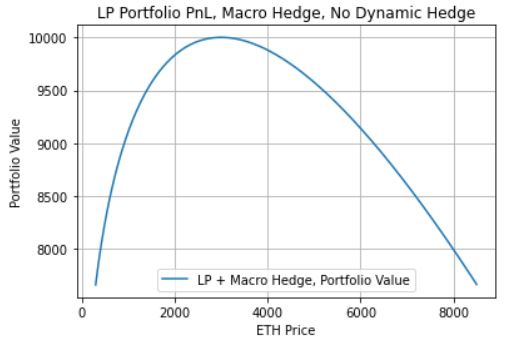
\includegraphics{LP_PnL_Macro}
\caption{PnL as a function of Spot Price for a macro-hedged LP Portfolio}
\label{fig:lp_pnl_macro}
\end{figure}

Differentiating this we get the delta of the portfolio required for our IL delta hedges
\begin{align}
\delta = 0.5 \; {\frac {C(0)} {p(0)}} \; {\frac {1 - \sqrt{x}}{\sqrt{x}}}
\label{eqn:delta_portfolio}
\end{align}
And at every rehedging time, we adjust our delta hedge to equal this. Some example price paths are shown in Fig.~\ref{fig:lp_pnl_dynamic} along with the corresponding portfolio IL with and without the dynamic hedge applied (but in all cases with the macro hedge applied). The PnL from the dynamically hedged portfolios is close to identical in all cases, despite the drastic differences in the ETH price paths and the PnL of the corresponding portfolios with only the macro hedge.

\begin{figure}
\centering
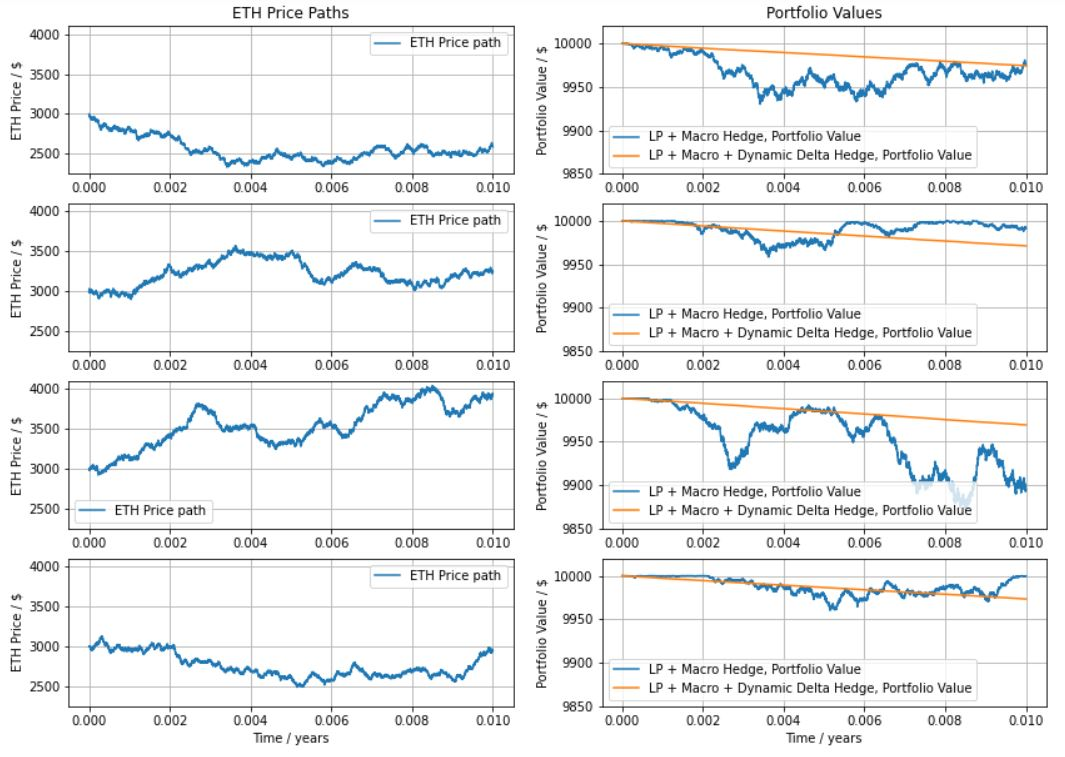
\includegraphics[scale=0.6]{LP_PnL_Dynamic2}
\caption{PnL as a function of Spot Price for a macro-hedged LP Portfolio. Note that different paths lead to very different PnL profiles for the macro-hedged-only portfolios, but the dynamically delta hedged portfolios display almost identical performance in all cases}
\label{fig:lp_pnl_dynamic}
\end{figure}

How frequently we should re-hedge is a good question. In a Black-Scholes style world with constant volatility parameter and zero costs, we can re-hedge very frequently and reduce the volatility of our PnL (although it will still be negative). In the real world, we have hedging costs, block times, and short-term vs. long-term volatility to think about. Out of scope for now.

We see from the delta hedging strategies discussed before that we expect to generate a approximately deterministic loss from the dynamic hedge, which is very standard for negative convexity portfolios. Again we make the crude Black-Scholes approximations, which risks dropping vol-of-vol cross terms etc. but gives us an intuitive idea of what is going on.

For a portfolio with gamma $\gamma$, the PnL for a dynamically delta-hedged portfolio is given by
\begin{align}
C(t, t+\Delta t) = 0.5 \; \gamma \; p(t)^2 \; \sigma^2 \; \Delta t
\label{eqn:gamma_pnl}
\end{align}
which is negative for a negative $\gamma$ portfolio, proportional to the time interval, and increases as $\sigma^2$ as vol $\sigma$ increases.

For the portfolio we've been considering so far, we can differentiate one more time to get the portfolio gamma
\begin{align}
\gamma = -0.25 \; {\frac {C(0)} {p(0)^2}} \; {\frac 1 {x^{3/2}}}
\label{eqn:gamma_portfolio}
\end{align}
The delta and gamma for the portfolio considered before are shown in Fig.~\ref{fig:lp_delta_gamma}.

\begin{figure}
\centering
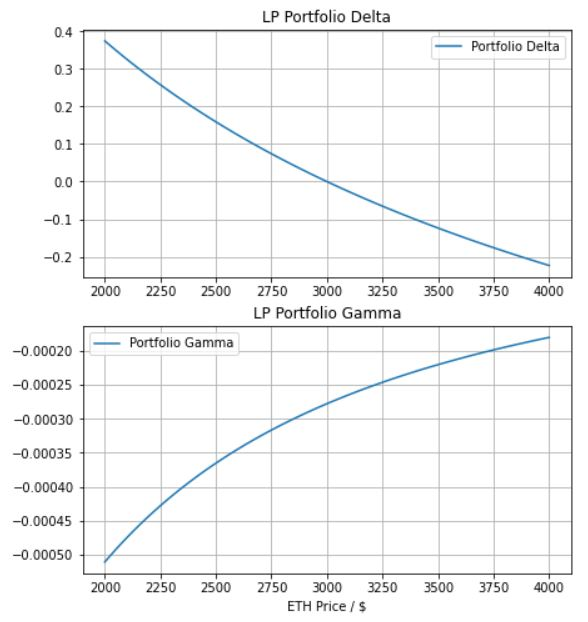
\includegraphics[scale=0.6]{LP_Delta_Gamma}
\caption{Portfolio delta and gamma for a macro-hedged LP Portfolio.}
\label{fig:lp_delta_gamma}
\end{figure}

We haven't talked about trading fees or governance token rewards, but of course we need these to match our negative gamma costs, or the cost of hedging out this gamma, for it to be worth staking coins.


\subsection*{Concentrated Liquidity}
\label{sec:concentrated}

UniSwap V3\footnote{https://uniswap.org/whitepaper-v3.pdf} and some other decentralized exchanges have introduced the concept of concentrated liquidity. The idea here is that in a constant factor AMM, you retain some combination of both coin X and coin Y all the way to infinite price. What if coin X was traded more quickly into coin Y as prices rose? More liquidity at lower prices would mean less slippage for traders, and a higher volume of trading in a tighter price range would mean more trading fees for liquidity providers.


\subsubsection*{UniSwap V3}

Within the UniSwap V3 framework, when providing liquidity LP stakers are required to also provide a range of prices $p_a < p_b$ between which their stake will be active. The constant factor AMM formula is adjusted for this `position' as follows
\begin{align}
\bigl( x + {\frac L {\sqrt{p_b}}} \bigr) \cdot ( y + L \sqrt{p_a} ) = L^2
\label{eqn:conc_liquidity}
\end{align}

When $p_a < p(t) \leq p_b$, this results in a greater amount of liquidity being provided for a similar amount of assets (and trading fees are now split between LPs according to liquidity provision rather than percentage of pool), and the position gamma is correspondingly larger as well. When $p(t)$ is outside of the range $p_a < p_b$, no liquidity is provided and no fees are earned. What is more, when $p < p_a$ the entire position has been converted into coin X, and when $p > p_b$ the entire position has been converted into coin Y.

At price $p(t)$, the quantity of coin X in the portfolio - which is also the size of the correct overall delta hedge at time $t$ (ie. macro hedge plus incremental hedge) - is
\begin{align}
x = L \Bigl( {\frac 1 {\sqrt{p(t)}}} - {\frac 1 {\sqrt{p_b}}} \Bigr)
\label{eqn:delta_hedge_conc}
\end{align}

The $\gamma$ coming from this derivative is the derivative of Eq.~\ref{eqn:delta_hedge_conc} wrt. price
\begin{align}
\gamma &= L {\frac {\partial} {\partial p(t)}} \Bigl( {\frac 1 {\sqrt{p(t)}}} - {\frac 1 {\sqrt{p_b}}} \Bigr) \\
&= -{\frac 1 2} L p(t)^{-{\frac 3 2}}
\label{eqn:gamma_conc}
\end{align}
which is exactly the same as the gamma of the unconcentrated position, except that it is multiplied by the larger liquidity factor $L$ coming from our concentration.

When we specify $p_a$ and $p_b$, depending upon the price we will no longer necessarily supply a constant value of both coin X and coin Y. But we can show that the value of both of these holdings will be equal exactly at the geometric center of the range, when
\begin{align*}
{\frac {y + L \sqrt{p_a}} {x + {\frac L {\sqrt{p_b}}}} } &= p(t) = {\frac y x} \\
x \cdot ( y + L \sqrt{p_a} ) &= y \cdot \bigl( x + {\frac L {\sqrt{p_b}}} \bigr) \\
x \cdot \sqrt{p_a} &= {\frac y {\sqrt{p_b}}} \\
p(t) &= \sqrt{p_a p_b}
\label{eqn:geometric_center}
\end{align*}

This raises an interesting question. Say we have 1 ETH and 3000 USDC and want to stake these in balanced quantities just as in the constant factor AMM case, but want to use concentrated liquidity to increase the liquidity we are supplying, what are the correct values of $p_a$ and $p_b$ to increase $L \to nL$?

In this case,
\begin{align*}
\bigl( x + {\frac L {\sqrt{p_b}}} \bigr) \cdot ( y + L \sqrt{p_a} ) &= n^2 L^2 = n^2 xy \\
\bigl( x + {\frac L {\sqrt{p_b}}} \bigr)^2 \sqrt{p_a p_b} &= n^2 x^2 \sqrt{p_a p_b} \\
x + {\frac L {\sqrt{p_b}}} &= nx \\
x + nx {\frac {\sqrt{\sqrt{p_a p_b}}} {\sqrt{p_b}}} &= nx \\
{\frac {p_a} {p_b}} &= \Bigl({\frac {n-1} n}\Bigr)^4
\end{align*}
which gives us
\begin{align}
p_a &= \Bigl({\frac {n-1} n}\Bigr)^2 p(t) \\
p_b &= \Bigl({\frac n {n-1}}\Bigr)^2 p(t)
\label{eqn:multiply_liquidity}
\end{align}
so for example to multiply the liquidity provided in the range by $10 \times$, we would need to choose $p_a = 0.81 \cdot p(t)$ and $p_b \simeq 1.2 \cdot p(t)$. This represents a considerable increase in the capital efficiency of the liquidity we are providing from our assets, at the cost of needing to actively manage our position should the price move outside of our liquidity range. Using concentration, we can `dial up' the gamma and the income we want for a position, while it stays within a set range of prices.

Examples of the Impermanent Loss and the $\gamma$ profiles of some example concentrated liquidity positions are shown in Fig.~\ref{fig:concentrated_liquidity_il_gamma}.

\begin{figure}
\centering
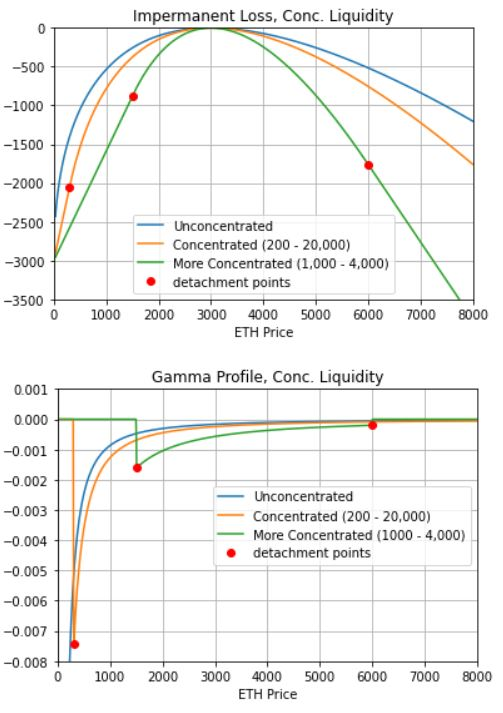
\includegraphics[scale=0.6]{Concentrated_Liquidity_IL_Gamma}
\caption{The IL and $\gamma$ profiles for some example concentrated liquidity positions all centered around $p=3000$ and initially composed of 1 ETH and 3000 USDC with a short macro hedge position of -1 ETH}
\label{fig:concentrated_liquidity_il_gamma}
\end{figure}


\subsubsection*{StableSwap}

Other liquidity concentration schemes also exist, the best-known of which is probably the StableSwap\footnote{https://curve.fi/files/stableswap-paper.pdf} algorithm used by curve.fi. This concentrates most of the liquidity into a very small part of the price axis and guarantees minimal slippage as long as prices stay within those bounds, which is very useful for stablecoin pairs and other highly correlated coins such as liquid staking tokens.

StableSwap chooses an invariant that blends `constant product' the `constant sum' liquidity. The invariant equation is
\begin{align}
A n^n \sum^n_1 x_i + D = A D n^n + {\frac {D^{n+1}} {n^n \; \prod^n_1 x_i}}
\label{eqn:stableswap}
\end{align}
where $x_i$ is the quantity of coin $i$ in the pool, $A$ controls the concentration of the pool, $n$ is the number of coins, and $D$ increases and decreases as liquidity is added and removed. Unlike UniSwap, this doesn't have analytical solutions but we can solve numerically for the behaviour and prices of each coin. The resulting pool makeup of a two coin pool as a function of concentration parameter $A$ is shown in Fig.~\ref{fig:stableswap}, we can see that as $A$ dials between very small and very large, we see the pool makeup curves vary from something that looks like a UniSwap constant factor model to a flat line between (2,0) and (0,2).

\begin{figure}
\centering
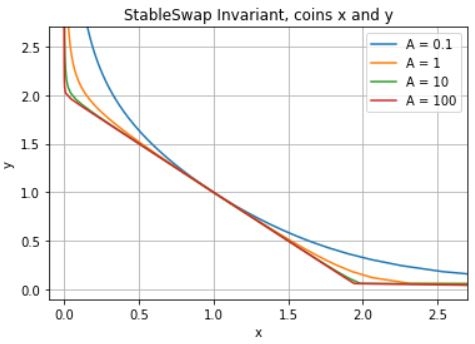
\includegraphics[scale=0.6]{StableSwap_Coin_Holdings}
\caption{The makeup of a two-coin StableSwap liquidity pool as a function of concentration parameter A}
\label{fig:stableswap}
\end{figure}

\begin{figure}
\centering
\includegraphics[scale=0.6]{StableSwap_Price_Quantity}
\caption{The price of coin x as pool holdings vary}
\label{fig:stableswap_price}
\end{figure}


\subsection*{Gamma Hedging}

There are a few approaches we can take to trying to hedge our gamma.

\begin{enumerate}

\item The `Vol Trader' View-on-Vol approach (ie. don't hedge it)

Trading volatility is all about having a view future realized vol that differs from the market's implied view\footnote{Volatility Trading, Euan Sinclair - https://www.amazon.com/Volatility-Trading-Website-Euan-Sinclair/dp/1118347137}.

If we believe the expression for gamma PnL given above, the yield for the LP staking is giving us the market's estimate of the price volatility that will be realized in the near future. If the market yield is currently $K$\% per year, the market is implying a vol of
\begin{align}
\sigma(t) = \sqrt{{\frac {K\; C(0)} {0.5 \; \gamma \; p(t)^2} }}
\label{eqn:implied_vol}
\end{align}
where $\sigma$ is the annualized volatility that will be realized over the next very short time window after time $t$. If our view is that the market is anticipating too much vol, it makes sense for us to sell it (ie. stake the coins).

Just to plug some numbers in for context, readily available yields on LP tokens from the market imply very high vols. A 30\% yield implies that it's worth staking coins unless the vol is likely to realize over 150\%...

Of course, the yield $K$\% is a spot yield, so we need to monitor this and be ready to withdraw liquidity if it no longer matches our view on vol.


\item Hedging with options

Hedging the gamma directly with options is tricky, because options gamma depends very sensitively on the spot price and the time to maturity, the gamma surface for a vanilla option with fixed vol of 50\% is shown in Fig.~\ref{fig:bs_gamma_surface}. Because of this, attempts to match the gamma (eg. with a straddle) will require expensive rehedging frequently.

\begin{figure}
\centering
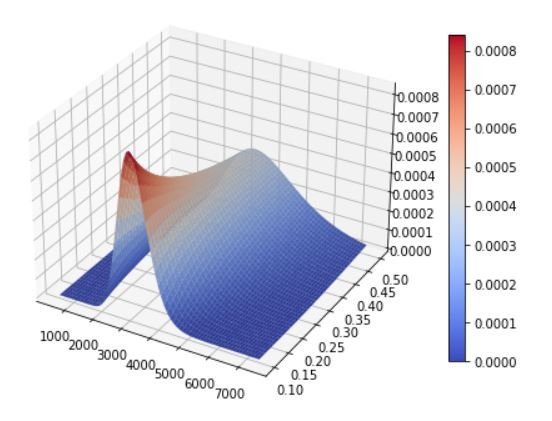
\includegraphics[scale=0.6]{BS_Gamma_Surface}
\caption{The $\gamma$ profile of an option in BS with spot=3000 and vol=50\% against strike price and time to maturity}
\label{fig:bs_gamma_surface}
\end{figure}

However, we know that if we have a continuum of option strikes available, we can statically replicate any fixed payoff at the same expiry, and even with a limited array of strikes we can do a reasonable job. Because of this, an alternative approach is to choose an options expiry date, then replicate the entire IL payoff function to that date. An example of this procedure is shown in Fig.~\ref{fig:lp_pnl_options}, where the strikes available on Deribit for expiry 4 days from now between \$2000 and \$4500 were used in the replication.

As we can see, for non-concentrated positions even with a limited selection of options available we are able to do a good job of replication within the price range, but the payoff rapidly diverges outside of our replication region. The situation is even more favourable for concentrated LP positions, where we are able to match the loss profile of the position both inside and outside of the cutoff regions.

\begin{figure}
\centering
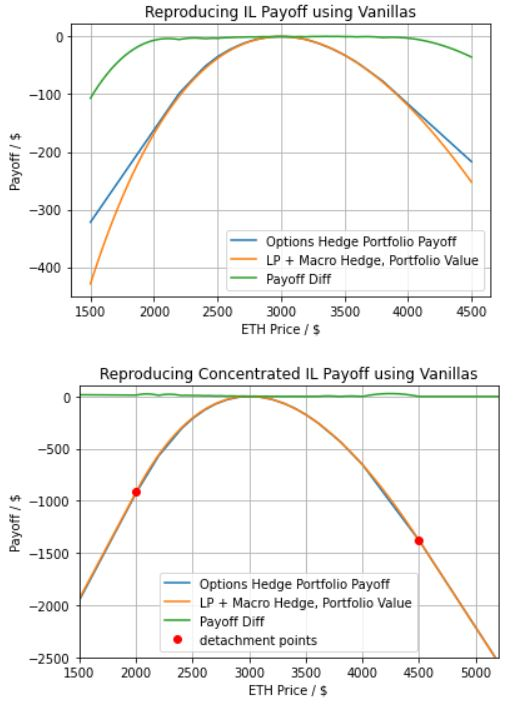
\includegraphics[scale=0.6]{LP_PnL_Options}
\caption{Replicating the payoff of two LP Portfolios worth \$10,000 at inception at a fixed time horizon using Options. The upper graph shows a non-concentrated LP position. Call strikes used were 3000, 3100, 3200, 3300, 3400, 3500, 3600, 3800 and corresponding ETH quantities were -0.01, -0.03, -0.03, -0.02, -0.02, -0.02, -0.03, -0.04; Put strikes used were 2200, 2400, 2500, 2600, 2700, 2800, 2900, 3000 and the corresponding ETH quantities were -0.09, -0.06, -0.04, -0.03, -0.03, -0.03, -0.03, -0.01. The lower graph shows a concentrated position of the same initial size with limit prices of \$2,000 and \$4,500. In this case, options are able to very nicely replicate the IL distribution even in the tails. Call strikes used were 3000, 3100, 3200, 3300, 3400, 3500, 3600, 3800, 4000, 4500 and the corresponding quantities were -0.07, -0.15, -0.13, -0.13, -0.13, -0.12, -0.17, -0.22, -0.33, -0.22; Pus strikes used were 2000, 2200, 2400, 2500, 2600, 2700, 2800, 2900, 3000 and the corresponding quantities were -0.27, -0.48, -0.32, -0.2, -0.18, -0.18, -0.17, -0.17, -0.08.}
\label{fig:lp_pnl_options}
\end{figure}

Advantages of this approach are that dynamic delta hedging will not be required and gamma is hedged to the expiry date. Disadvantages are that the portfolio will have mark-to-market PnL coming from the option portfolio vega as implied vol moves around so closing out early could involve loss, and at expiry a new hedge must be entered or the LP position closed.

I'm going to pull some deribit data to look at how much we might expect this to cost for different tenors, vs. the approximate yield we might expect to receive from the LP token in that time (COMING SOON), as this could be a nice little strategy when options are selling cheap\footnote{It's been suggested to me that with the rise of covered call selling vaults for yield enhancement via auctions, option prices might be getting suppressed particularly in the wings on auction dates. One example is the weekly options auction from Ribbon Finance, https://auction.ribbon.finance/, but I need to pull some more data for comprehensive testing}.


\item Hedging with Everlasting Options, Variance Swaps, ... (WORK IN PROGRESS)

To get around the expiry dates and need to roll hedges, we might be able to hedge with Everlasting Options\footnote{https://www.paradigm.xyz/2021/05/everlasting-options}. These won't avoid the vega PnL issues but do remove the need for us to roll our option hedge.

Variance Swaps are also an interesting thought. They have flat gamma at all prices and no delta exposure, so they would be able to hedge the initial level of our gamma but not its changes as spot moves. Variance swaps also have the vega PnL and expiry rolling issues we met with options.

Variance swaps don't really trade in crypto yet, and it's not clear how you'd index them without a good choice of `fixing time'. Once interesting possibility is that once could construct a volatility index using UniSwap itself, taking the price at the start or end of every block, along with the block timestamp, and use that to measure Variance Swap payoffs.

\end{enumerate}


\end{document}